% Options for packages loaded elsewhere
\PassOptionsToPackage{unicode}{hyperref}
\PassOptionsToPackage{hyphens}{url}
%
\documentclass[
  9pt,
  ignorenonframetext,
]{beamer}
\usepackage{pgfpages}
\setbeamertemplate{caption}[numbered]
\setbeamertemplate{caption label separator}{: }
\setbeamercolor{caption name}{fg=normal text.fg}
\beamertemplatenavigationsymbolsempty
% Prevent slide breaks in the middle of a paragraph
\widowpenalties 1 10000
\raggedbottom
\setbeamertemplate{part page}{
  \centering
  \begin{beamercolorbox}[sep=16pt,center]{part title}
    \usebeamerfont{part title}\insertpart\par
  \end{beamercolorbox}
}
\setbeamertemplate{section page}{
  \centering
  \begin{beamercolorbox}[sep=12pt,center]{part title}
    \usebeamerfont{section title}\insertsection\par
  \end{beamercolorbox}
}
\setbeamertemplate{subsection page}{
  \centering
  \begin{beamercolorbox}[sep=8pt,center]{part title}
    \usebeamerfont{subsection title}\insertsubsection\par
  \end{beamercolorbox}
}
\AtBeginPart{
  \frame{\partpage}
}
\AtBeginSection{
  \ifbibliography
  \else
    \frame{\sectionpage}
  \fi
}
\AtBeginSubsection{
  \frame{\subsectionpage}
}
\usepackage{lmodern}
\usepackage{amsmath}
\usepackage{ifxetex,ifluatex}
\ifnum 0\ifxetex 1\fi\ifluatex 1\fi=0 % if pdftex
  \usepackage[T1]{fontenc}
  \usepackage[utf8]{inputenc}
  \usepackage{textcomp} % provide euro and other symbols
  \usepackage{amssymb}
\else % if luatex or xetex
  \usepackage{unicode-math}
  \defaultfontfeatures{Scale=MatchLowercase}
  \defaultfontfeatures[\rmfamily]{Ligatures=TeX,Scale=1}
\fi
\usetheme[]{Goettingen}
\usecolortheme{rose}
% Use upquote if available, for straight quotes in verbatim environments
\IfFileExists{upquote.sty}{\usepackage{upquote}}{}
\IfFileExists{microtype.sty}{% use microtype if available
  \usepackage[]{microtype}
  \UseMicrotypeSet[protrusion]{basicmath} % disable protrusion for tt fonts
}{}
\makeatletter
\@ifundefined{KOMAClassName}{% if non-KOMA class
  \IfFileExists{parskip.sty}{%
    \usepackage{parskip}
  }{% else
    \setlength{\parindent}{0pt}
    \setlength{\parskip}{6pt plus 2pt minus 1pt}}
}{% if KOMA class
  \KOMAoptions{parskip=half}}
\makeatother
\usepackage{xcolor}
\IfFileExists{xurl.sty}{\usepackage{xurl}}{} % add URL line breaks if available
\IfFileExists{bookmark.sty}{\usepackage{bookmark}}{\usepackage{hyperref}}
\hypersetup{
  pdftitle={BIOS6643 Longitudinal},
  pdfauthor={EJC},
  hidelinks,
  pdfcreator={LaTeX via pandoc}}
\urlstyle{same} % disable monospaced font for URLs
\newif\ifbibliography
\setlength{\emergencystretch}{3em} % prevent overfull lines
\providecommand{\tightlist}{%
  \setlength{\itemsep}{0pt}\setlength{\parskip}{0pt}}
\setcounter{secnumdepth}{-\maxdimen} % remove section numbering
\AtBeginSubsection{}
\AtBeginSection{}
\ifluatex
  \usepackage{selnolig}  % disable illegal ligatures
\fi

\title{BIOS6643 Longitudinal}
\subtitle{L11 Nesting and Cross II}
\author{EJC}
\date{}
\institute{Department of Biostatistics \& Informatics}

\begin{document}
\frame{\titlepage}

\begin{frame}[allowframebreaks]
  \tableofcontents[hideallsubsections]
\end{frame}
\hypertarget{nesting-and-cross}{%
\section{Nesting and Cross}\label{nesting-and-cross}}

\begin{frame}{Topics for this lecture:}
\protect\hypertarget{topics-for-this-lecture}{}
\begin{itemize}
\tightlist
\item
  Nesting and crossing (2nd day)
\end{itemize}

\vspace{\baselineskip}

\begin{itemize}
\item
  \textbf{Associated reading: Course notes}

  \begin{itemize}
  \item
    `Nesting and crossing' section in LMM chapter
  \item
    Hedeker, Ch. 13 (for hierarchical models).
  \end{itemize}
\end{itemize}
\end{frame}

\hypertarget{case-study}{%
\section{Case study}\label{case-study}}

\begin{frame}{Mouse and tumor data}
\protect\hypertarget{mouse-and-tumor-data}{}
\begin{itemize}
\item
  Consider an experiment performed at the university involving trials on
  mice (Dr.~Kian Behbakht, PI).

  \begin{itemize}
  \item
    Each mouse in the experiment was assigned to receive a treatment (A,
    B, Control), and then two tumors were planted within each mouse.
  \item
    Tumor volume measurements (unspecified units) were then taken five
    times on each tumor.
  \item
    For these data,
  \end{itemize}

  \begin{enumerate}
  \tightlist
  \item
    the mouse is the level-3 data;
  \item
    tumors within mice are level-2 data, 3.the repeated measures are
    level-1 data.
  \end{enumerate}
\end{itemize}
\end{frame}

\begin{frame}{}
\protect\hypertarget{section}{}
\begin{itemize}
\item
  Treatment A and B tend to actually maintain the tumor size, while
  those in the Control tend to have tumors that shrink over time.
  However whether these differences are significant remains to be seen,
  and is the purpose for fitting a linear mixed model.
\item
  The units follow a 3-level nested pattern, however information was not
  provided on whether tumors were systematically placed within mice
  (e.g.~`Tumor 1' on left and `Tumor 2' on right), or just randomly
  placed.
\item
  The units can be considered nested, with 3 levels. However, it is not
  clear whether the tumor and mouse should be considered nested or
  crossed factors.
\end{itemize}
\end{frame}

\begin{frame}{}
\protect\hypertarget{section-1}{}
Let's consider 2 possible modeling approaches for repeated measures:

\begin{itemize}
\item
  \textbf{Approach 1}: consider tumor as nested within mouse; include
  nested random effects plus an error covariance structure for repeated
  measures over time.

  \begin{itemize}
  \item
    Recall that including a random effect at one level will induce
    correlation between units on the next lower level. (E.g., including
    a random intercept for subjects induces correlation on the repeated
    measures within subjects.)
  \item
    By including random effects for mouse and tumor, we have modeled
    correlation between tumors and between times.
  \end{itemize}
\item
  \textbf{Approach 2}: Assume tumors were placed systematically within
  mice, so that tumor and time can be considered as crossed factors, and
  use the Kronecker Product structure.
\end{itemize}
\end{frame}

\begin{frame}{}
\protect\hypertarget{section-2}{}
\begin{itemize}
\item
  Even if tumors and time were not actually crossed, Approach 2 yields a
  reasonable approximate covariance structure for Yi. In particular,
  this modeling approach results in a structure that makes intuitive
  sense since it allows for a decay in correlation between tumor
  measurements within a mouse, as time between measurements is
  increased. Approach 1 does not allow for this.
\item
  Final analyses were performed on log transformed tumor volumes for two
  reasons:

  \begin{itemize}
  \item
    \begin{enumerate}
    [(i)]
    \tightlist
    \item
      log volumes were more normally distributed
    \end{enumerate}
  \item
    \begin{enumerate}
    [(i)]
    \setcounter{enumi}{1}
    \tightlist
    \item
      results were not as sensitive to model specifications, e.g.,
      `Approach 1' (A1) versus `Approach 2' (A2).
    \end{enumerate}
  \end{itemize}
\item
  The structures for these modeling approaches are shown below, followed
  by actual fits with the data. To simplify notation, I considered 3
  repeated measures within mice rather than 5. For actual fits, what
  complicates matters is that only Treatment B had all 3 mice with 2
  tumors measured; the other groups only had 1 of 3 mice with 2 tumors
  measured (the remaining mice just had 1).
\end{itemize}
\end{frame}

\begin{frame}{SAS code}
\protect\hypertarget{sas-code}{}
Here is the SAS code to carry out model fits for the approaches,
followed by more detail for each one.

\begin{center}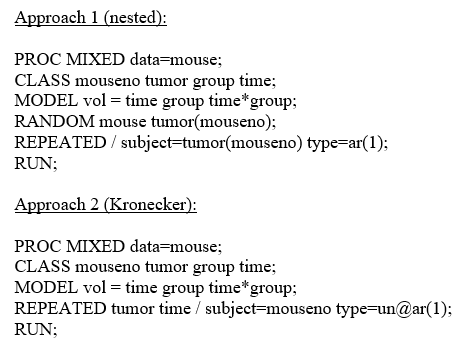
\includegraphics[width=0.7\linewidth]{figs_L11/f1} \end{center}
\end{frame}

\hypertarget{approach-1}{%
\section{Approach 1}\label{approach-1}}

\begin{frame}{Approach 1:}
\protect\hypertarget{approach-1-1}{}
Consider tumors as nested within mice, and repeated measures as nested
within tumors (3-level data).

The model can be expressed as
\(Y_{hij}=\pmb x_{hij} {\pmb \beta}+b_h+b_{i(h)}+\epsilon_{hij}\), where
\(b_h\sim \mathcal N(0,\sigma_M^2)\),
\(b_{i(h)}\sim \mathcal N(0,\sigma_T^2)\) and \(\epsilon_{hij}\) follows
an AR(1) process (within tumor), other; \(h\), \(i\) and \(j\) index
mouse, tumor and measure, respectively.

For practice, write out the design matrix for the random effects for
largest unit, mouse: \(\pmb Z_h\), and for the full data: \(\pmb Z\).

The resulting \(\pmb V_h\) matrix would be:

\begin{center}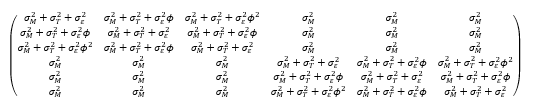
\includegraphics[width=1\linewidth]{figs_L11/f0} \end{center}

One of the problems that I have with this structure is that the
covariance for measurements between tumors at different times stays the
same as the times are more spread out.
\end{frame}

\begin{frame}{Results}
\protect\hypertarget{results}{}
Model fit: AIC=188.5. This model estimates that there is no covariance
between tumors within mice.

\begin{center}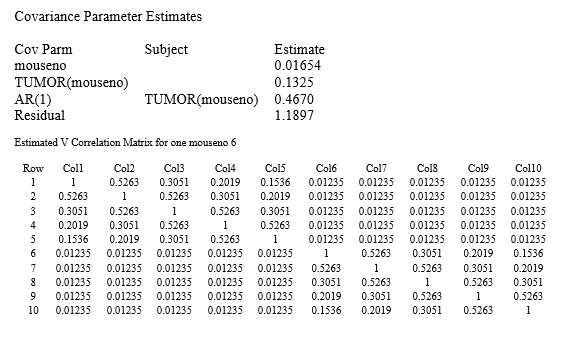
\includegraphics[width=1\linewidth]{figs_L11/f2} \end{center}
\end{frame}

\hypertarget{approach-2}{%
\section{Approach 2}\label{approach-2}}

\begin{frame}{Approach 2:}
\protect\hypertarget{approach-2-1}{}
Kronecker Product structure, using the UN structure for tumors within
mice, and repeated measures over time using the AR(1) structure.

The model is \(Y_{hij}=x_{hij} {\pmb \beta}+\epsilon_{hij}\), where
\(h\) indexes mouse, \(i\) indexes tumor and \(j\) indexes time,
\(x_{hij}\) is a row vector containing the predictors. We will consider
covariance structures relative to `mouse' (with index \(h\)), since that
is the largest experimental unit. Thus, we need to derive R\_h, the
covariance matrix for vector \(\epsilon_h\).

Structure for 2
tumors:\(R_{h1}=\begin{pmatrix} \sigma_1^2 & \sigma_{12} \\ \sigma_{12} & \sigma_2^2 \end{pmatrix}\)
3 times:
\(R_{h2}=\sigma_\epsilon^2 \begin{pmatrix} 1 & \phi & \phi^2 \\ \phi&1 & \phi \\ \phi^2 & \phi&1 \end{pmatrix}\)
\end{frame}

\begin{frame}{}
\protect\hypertarget{section-3}{}
The combined (Kronecker product structure):

\[
\pmb R_h = R_{h1} \otimes R_{h2} =
\begin{pmatrix}
\sigma_1^2 & \sigma_1^2 \phi & \sigma_1^2 \phi^2 & \sigma_{12}  & \sigma_{12}  \phi & \sigma_{12}  \phi^2  \\
\sigma_1^2 \phi & \sigma_1^2 & \sigma_1^2 \phi & \sigma_{12}  \phi & \sigma_{12}  & \sigma_{12}  \phi  \\ 
\sigma_1^2 \phi^2 & \sigma_1^2 \phi & \sigma_1^2 & \sigma_{12}  \phi^2 & \sigma_{12}  \phi & \sigma_{12}   \\  
\sigma_{12}  & \sigma_{12}  \phi & \sigma_{12}  \phi^2 & \sigma_2^2 & \sigma_2^2 \phi & \sigma_2^2 \phi^2  \\  
\sigma_{12}  \phi & \sigma_{12}  & \sigma_{12}  \phi & \sigma_2^2 \phi & \sigma_2^2 & \sigma_2^2 \phi  \\ 
\sigma_{12}  \phi^2 & \sigma_{12}  \phi & \sigma_{12}  & \sigma_2^2 \phi^2 & \sigma_2^2 \phi & \sigma_2^2 
\end{pmatrix} = \pmb V_h
\]

The \(\sigma_\epsilon^2\) on the AR(1) structure is not included because
it becomes redundant once we take the direct product, i.e., it is
absorbed into parameters in the other matrix.
\end{frame}

\begin{frame}{Results}
\protect\hypertarget{results-1}{}
Model fit: AIC=188.1. Here, we get a covariance between tumors within
mice that decays as the time between measurements is increased.

\begin{center}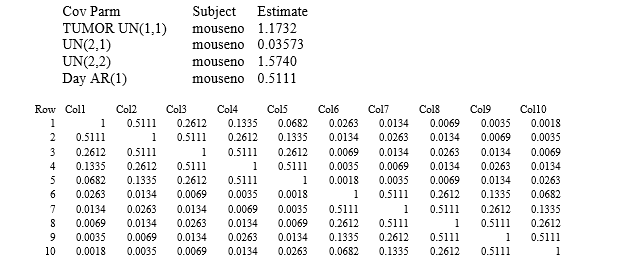
\includegraphics[width=1\linewidth]{figs_L11/f3} \end{center}
\end{frame}

\begin{frame}{Comparison}
\protect\hypertarget{comparison}{}
Although the model fits have similar AIC values, Approach 2 yields a
slightly better model fit; approaches have the same number of covariance
parameters (there is no `simpler' model).

Below is full SAS code and some of the tests of interest for Approach 2.
The PI for the project had specifically asked for a comparison of groups
at the last time (time 18).

\begin{center}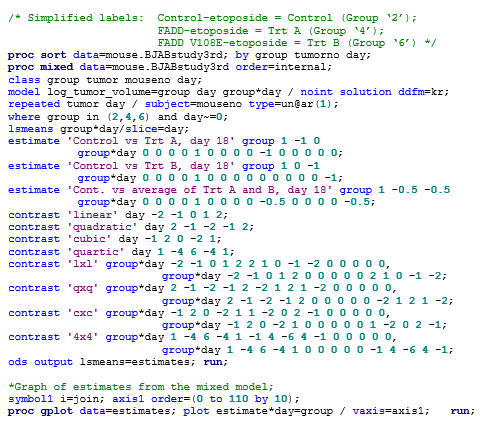
\includegraphics[width=0.7\linewidth]{figs_L11/f4} \end{center}
\end{frame}

\begin{frame}{Abbreviated output:}
\protect\hypertarget{abbreviated-output}{}
\begin{center}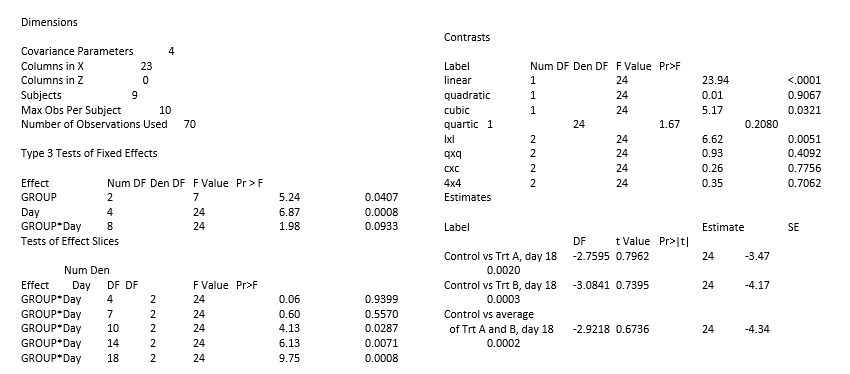
\includegraphics[width=1\linewidth]{figs_L11/f5} \end{center}
\end{frame}

\begin{frame}{}
\protect\hypertarget{section-4}{}
\begin{center}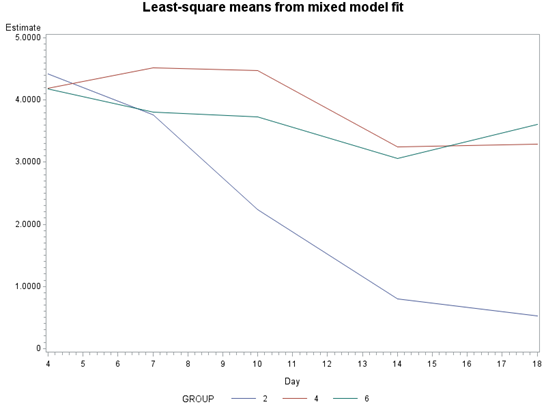
\includegraphics[width=0.5\linewidth]{figs_L11/f6} \end{center}

There is a general cubic pattern (flattish, drop, flattish), but since
this pattern exists more or less for each group (after accounting for
linear trends), we do not see a cubic-by-cubic interaction.

There is a clear linear trend as well as linear-by-linear interaction.

Finally, control differs significantly from each of the other groups,
particularly at later times. Mean log volume for control was
significantly different than Treatments A and B at 18 days.
\end{frame}

\hypertarget{discussion}{%
\section{Discussion}\label{discussion}}

\begin{frame}{Discussion}
\protect\hypertarget{discussion-1}{}
If the design is really a nested one and tumors are not crossed but the
Kronecker Product structure is still used as an approximate model, it
may make more sense to use CS \(\otimes\) AR(1). (If tumors `1' and `2'
are arbitrarily assigned across mice, we probably wouldn't want to use
separate variances for them, such as is done with the UN structure.)
However, right now SAS does not have a canned structure for that. Thus,
we are probably spending an extra DF for no real reason. Nevertheless,
we only have 4 covariance parameters, and it's the same number used for
Approach 1. Hopefully later versions will have that capability.

In general I would recommend that you stick with the model that is
consistent with the design UNLESS there is good reason to change.

For this study, we were not completely sure of the design. If this were
going into a publication, I would definitely discuss more with the PI.
However, Approach 2 yields a reasonable and intuitive structure even if
the tumors were not systematically placed within mice (particularly if a
CS \(\otimes\) AR(1) structure could easily be programmed).
\end{frame}

\hypertarget{crossover-designs-for-repeated-measures-data}{%
\section{Crossover designs for repeated measures
data}\label{crossover-designs-for-repeated-measures-data}}

\begin{frame}{Crossover designs for repeated measures data}
\protect\hypertarget{crossover-designs-for-repeated-measures-data-1}{}
In some cases a researcher may want to have each subject try multiple
treatments in an experiment, rather than just one. In the simplest case,
there are 2 treatments, which can be assigned to each subject in a 2
period, 2 treatment (2 \(\times\) 2) crossover design.

For the 2 \(\times\) 2 design, subjects are usually randomly assigned an
order of treatments, AB or BA, in equal amount. This helps to eliminate
confounders associated with time.

If there are 3 treatments, then one may set up a 3 period, 3 treatment
crossover design.

Crossover designs are often used in clinical trials when the cost of
tracking subjects longitudinally for extended time does not impose major
difficulties.
\end{frame}

\begin{frame}{Carry-over}
\protect\hypertarget{carry-over}{}
\textbf{Carry-over effects}: One limitation of crossover designs is that
receiving one treatment first may have an influence on subjects'
responses in the subsequent period in which they receive the other
treatment.

\begin{itemize}
\item
  If this carry-over effect differs between treatment sequences, then
  estimates of effect of interest may be biased.
\item
  The difficulty with the 2 \(\times\) 2 design is that carry-over
  effect estimates are aliased with other effects (i.e., they are
  completely confounded with each other). Specifically, the sequence,
  carry-over and period*treatment effects are aliased.
\item
  If sequence and period*treatment effects are assumed to not exist,
  then we can test for carry-over effects by including the sequence term
  in the model. But the validity of the test relies on that
  assumption\ldots{}
\item
  In more complex models, it is easier to estimate carryover effects by
  examining interactions. Including a term in the model for treatment
  used in the previous period may help in estimating (differential)
  carryover effects.
\end{itemize}
\end{frame}

\begin{frame}{}
\protect\hypertarget{section-5}{}
\begin{itemize}
\item
  For any crossover design, including a washout period of suitable
  length between treatment periods may help to eliminate carryover
  effects that a treatment might have. Most researchers do include some
  washout period in their crossover experiment, however one of the
  issues that arises is planning in advance how long this should be
  since it is often uncertain how long it will take to `wash out' the
  treatment.
\item
  If some carryover effects are expected for a given study or
  experiment, then the researcher may also consider using alternative
  designs. Here, we focus on crossover experiments with repeated
  measures within periods.
\item
  For more examples and details about modeling data from crossover
  designs, see \textbf{Littell et al, SAS System for Mixed Models}, and
  \textbf{Jones and Kenward, Design and Analysis of Cross-Over Trials}
  (in particular, see Chapter 5).
\end{itemize}
\end{frame}

\begin{frame}{}
\protect\hypertarget{section-6}{}
Consider a crossover experiment that was performed and reported in
\textbf{Connolly et al.~(2006)}, entitled \emph{Efficacy of a tart
cherry juice blend in preventing the symptoms of muscle damage (British
Journal of Sports Medicine, 40: 679-683)}.

\begin{itemize}
\item
  In the experiment, subjects were randomized to receive cherry juice
  twice a day or placebo drink for 8 consecutive days.
\item
  At day 4, subjects performed `eccentric elbow flexion contractions'.
\item
  Measures of strength and pain after the challenge (relative to
  baseline) were then taken on subjects on the last 4 days of the
  period, after the challenge.
\item
  Subjects then repeated the experiment with the treatment they did not
  have in Period 1, using the opposite arm. Mean strength was greater
  and pain was less when subjects had the cherry drink, relative to
  placebo. Strength loss relative to BL was 22\% for placebo but only
  4\% for cherry juice.
\item
  This is considered a 2-period, 2-treatment crossover design, with
  repeated measures.
\end{itemize}
\end{frame}

\begin{frame}{}
\protect\hypertarget{section-7}{}
In the spirit of this experiment, consider a hypothetical data set
involving muscle soreness measurements on 4 successive days after an
exercise challenge. This soreness score ranges from 0 to 10 but is
typically in a range of 1 to 4. These scores are adjusted for baseline
soreness before the experiment (e.g., if a subject has a soreness score
of 2 coming into the study and a score of 6 one day after the challenge,
then their soreness score on that day would be 4). This was designed
like the reported experiment (2 \(\times\) 2 crossover, 4 repeated
measures within each period).
\end{frame}

\begin{frame}{}
\protect\hypertarget{section-8}{}
Below is a description of the predictors in the model and what they can
be used to test:

\begin{itemize}
\tightlist
\item
  \textbf{Period:} 1 or 2; test accounts for differences between first
  and second time periods.
\item
  \textbf{Treatment:} placebo vs.~cherry drink; test is for main effect
  of treatment (comparing treatment means).
\item
  \textbf{Time:} the 4 days that measures were taken following the
  exercise challenge; test is for main effect of time (comparing means
  for 4 days following the exercise challenge); time modeled as a class
  variable.
\item
  \textbf{Period \(\times\) time:} Will test for differences between
  time patterns between the two periods. Can be thought of as the
  general time variable.
\item
  \textbf{Treatment \(\times\) time:} Will test whether changes over
  time (with a period) differ between the placebo and cherry drink. If
  treatment \(\times\) time is significant, then comparisons can be made
  between treatments for individual days (with multiple comparison
  adjustments, if desired).
\item
  \textbf{Sequence:} Compares AB versus BA treatments. Since there are
  only 2 treatments, this sequence effect is aliased with carry-over
  effects. We can use this term to test for carry-over effects assuming
  that there are no true treatment \(\times\) period or (other) sequence
  effects.
\end{itemize}
\end{frame}

\begin{frame}{Here is the SAS code for the analysis.}
\protect\hypertarget{here-is-the-sas-code-for-the-analysis.}{}
\begin{center}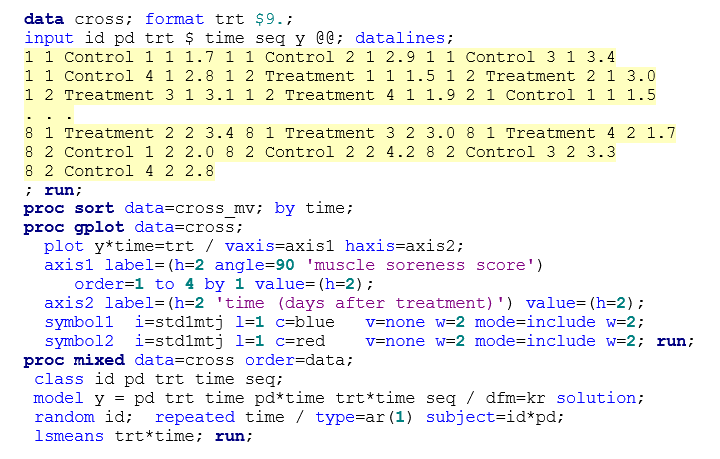
\includegraphics[width=1\linewidth]{figs_L11/f7} \end{center}
\end{frame}

\begin{frame}{Abbreviated output:}
\protect\hypertarget{abbreviated-output-1}{}
\begin{center}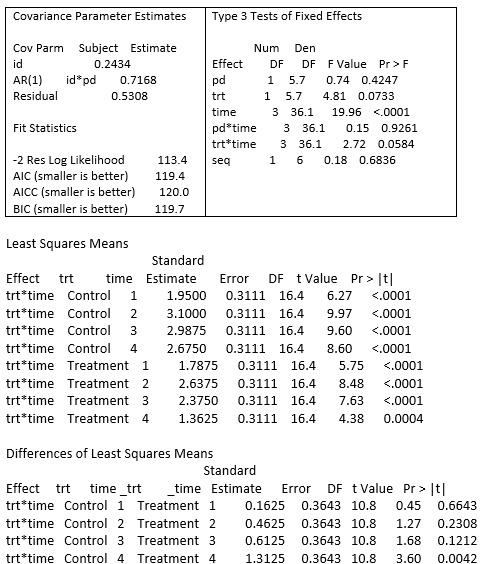
\includegraphics[width=0.7\linewidth]{figs_L11/f8} \end{center}

\alert {Interpretations of the results?}
\end{frame}

\begin{frame}{Graph of sample means and SD error bars.}
\protect\hypertarget{graph-of-sample-means-and-sd-error-bars.}{}
\begin{center}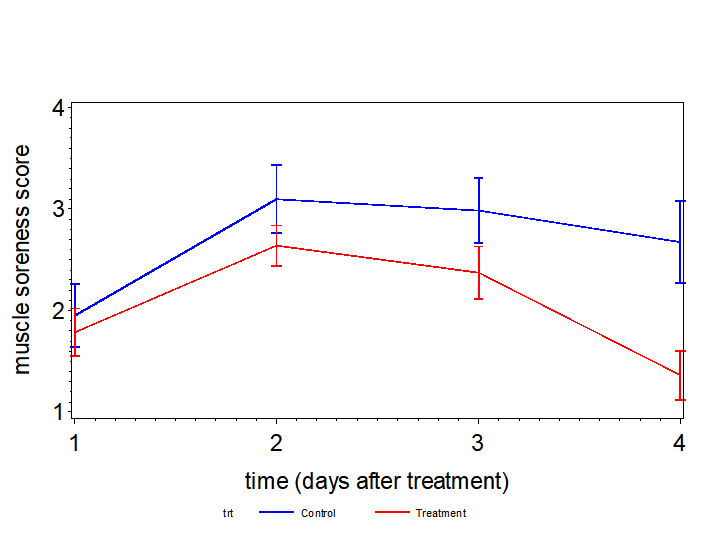
\includegraphics[width=1\linewidth]{figs_L11/f9} \end{center}

\textbf{Another example:} sleep study I conducted, where kids had
`short' and `long' sleep weeks.

Similar crossover design with washout.
\end{frame}

\end{document}
